\documentclass{VUMIFPSbakalaurinis}
\usepackage{algorithmicx}
\usepackage{algorithm}
\usepackage{algpseudocode}
\usepackage{amsfonts}
\usepackage{amsmath}
\usepackage{bm}
\usepackage{caption}
\usepackage{color}
\usepackage{float}
\usepackage{graphicx}
\usepackage{listings}
\usepackage{subfig}
\usepackage{wrapfig}
\usepackage[table,xcdraw]{xcolor}
\usepackage{enumitem}
\usepackage{longtable}
\setitemize{noitemsep,topsep=0pt,parsep=0pt,partopsep=0pt}
\setenumerate{noitemsep,topsep=0pt,parsep=0pt,partopsep=0pt}

\hbadness=100000
% Titulinio aprašas
\university{Vilniaus universitetas}
\faculty{Matematikos ir informatikos fakultetas}
\department{Programų sistemų studijų programa}
\papertype{Mokslo tiriamasis darbas III}
\title{Srautinio apdorojimo sistemų balansavimas taikant mašininį mokymąsi}
\titleineng{Balancing stream processing systems using machine learning}
\author{Vytautas Žilinas}
\supervisor{Andrius Adamonis}
\reviewer{Prof. dr. Aistis Raudys}
\date{Vilnius – \the\year}

% Nustatymai
% \setmainfont{Palemonas}   % Pakeisti teksto šriftą į Palemonas (turi būti įdiegtas sistemoje)
\bibliography{bibliografija}

\begin{document} 
\maketitle

\cleardoublepage\pagenumbering{arabic}
\setcounter{page}{2}

\tableofcontents

\sectionnonum{Įvadas}

Realaus laiko duomenų apdorojimas (angl. real–time data processing) yra jau senai nagrinėjamas kaip vienas iš būdų apdoroti didelių kiekių duomenis (angl. Big data). Viena iš didelių duomenų apdorojimo tipinių architektūrų yra srautinis apdorojimas. Srautinis duomenų apdorojimas (angl. stream processing) – lygiagrečių programų kūrimo modelis, pasireiškiantis sintaksiškai sujungiant nuoseklius skaičiavimo komponentus srautais, kad kiekvienas komponentas galėtų skaičiuoti savarankiškai \cite{shortstreamproc}. 

Yra keli pagrindiniai srautinio apdorojimo varikliai: „Apache Storm“, „Apache Spark“, „Heron“ ir kiti. „Apache Storm“ ir „Heron“ apdoroja duomenis duomenų srautais, o „Apache Spark“ mikro–paketais \cite{karau2015learning}. „Heron“ srautinio apdorojimo variklis, buvo išleistas „Twitter“ įmonės 2016 metais kaip patobulinta alternatyva „Apache Storm“ srautinio apdorojimo varikliui \cite{openSourcing}. Šiame darbe bus naudojamas „Heron“, kadangi tai yra naujesnis ir greitesnis srautinio apdorojimo variklis nei „Apache Storm“ \cite{twitterHeron}. 

Srautinio apdorojimo sistemų balansavimas (angl. auto–tuning) – tai sistemos konfigūracijos valdymas siekiant užtikrinti geriausią resursų išnaudojimą – duomenų apdorojimas neprarandant greičio, bet ir naudojant tik reikiamą kiekį resursų. Kadangi srautinio apdorojimo sistemų komponentai yra kuriami kaip lygiagretus skaičiavimo elementai, todėl jie gali būti plečiami horizontaliai ir vertikaliai \cite{shortstreamproc} keičiant sistemų konfigūraciją. Tačiau lygiagrečių elementų kiekio keitimas nėra vienintelis būdas optimizuoti resursų išnaudojimą. Kiekvienas variklis turi savo rinkinį konfigūruojamų elementų. Pavyzdžiui, darbe naudojamas „Heron“ variklis leidžia optimizuoti sistemas naudojant 56 konfigūruojamus parametrus \cite{configDocument}.

Yra skirtingi būdai kaip gali būti parenkama tinkama konfigūracija. Kadangi srautinio apdorojimo sistemų apkrovos gali būti skirtingų pobūdžių (duomenų kiekis, skaičiavimų sudėtingumas, nereguliari apkrova), o inžinieriai kurdami ir konfigūruodami taikomąsias sistemas išbando tik kelis derinius ir pasirenka labiausiai tinkanti \cite{selfRegulatingStreaming}, lieka daug skirtingų neišbandytų konfigūracijos variacijų. Optimalios konfigūracijos suradimas yra NP sudėtingumo problema \cite{automateTuning}, kadangi žmonėms yra sunku suvokti didelį kiekį konfigūracijos variacijų. 
Vienas iš būdų automatiškai valdyti konfigūraciją buvo pasiūlytas 2017 metų straipsnyje „Dhalion: self–regulating stream processing in heron“, kuriame autoriai aprašo savo sukurtą sprendimą „Dhalion“, kuris konfigūruoja „Heron“ srautinio apdorojimo sistemas pagal esamą apkrova ir turimus resursus, tai yra jei apdorojimo elementų išnaudojimas išauga virš 100\%, „Dhalion“ padidina lygiagrečiai dirbančių apdorojimo elementų kiekį \cite{dhalion}. Tačiau toks sprendimas leidžia reguliuoti tik elementų lygiagretumą ir tai daro tik reaktyviai.

Vienas iš naujausių būdų balansuoti srautinio apdorojimo sistemas – mašininis mokymasis. Vienas iš tokių bandymų aprašytas 2018 metų straipsnyje „Auto–tuning Distributed Stream Processing Systems using Reinforcement Learning“\cite{vaquero2018autotuning} kuriame atliktas tyrimas – „Apache Spark“ sistemos balansavimui naudojamas skatinamojo mokymo REINFORCE algoritmas, kuris, pagal dabartinę konfigūraciją ir renkamas metrikas, keitė srautinio apdorojimo sistemos konfigūracijos parametrus. Šiame tyrime pasiūlytas sprendimas, naudojantis mašininį mokymąsi, suranda efektyvesne konfigūraciją per trumpesnį laiką nei žmonės, o tokiu būdu išskaičiuotą konfigūraciją naudojanti sistema pasiekia 60–70\% mažesnį vėlinimą, nei naudojanti ekspertų rankiniu būdu nustatytą konfigūraciją. \cite{vaquero2018autotuning}. Šiame darbe naudojamas „Heron“ variklis leidžia prie savęs prijungti sukurtą išorinę metrikų surinkimo programą, kuri gali rinkti tokias sistemų metrikas kaip: naudojama RAM atmintis, CPU apkrova, komponentų paralelizmas ir kitas, kurios gali būti naudojamos balansavimui. 

Skatinamasis mokymasis yra vienas iš mašininio mokymosi tipų. Šis mokymasis skiriasi nuo kitų, nes nereikia turėti duomenų apmokymui, o programos mokosi darydamos bandymus ir klysdamos. Vienas iš pagrindinių privalumų naudojant skatinamąjį mokymąsi balansavimui – nereikia turėti išankstinių duomenų apmokymui, kas leidžia jį paprasčiau pritaikyti skirtingoms srautinio apdorojimo sistemų apkrovoms. Tačiau tokio tipo mašininis mokymasis turi ir problemų: sudėtinga aprašyti tinkamos konfigūracijos apdovanojimo (angl. reward) funkciją ir balansą tarp tyrinėjimo ir išnaudojimo tam, kad nebūtų patiriami nuostoliai \cite{selfRegulatingStreaming}.

Yra sukurta daug skatinamojo mokymosi algoritmų (Monte Carlo, Q–learning, Deep Q Network ir kiti), šiame darbe jie apžvelgti, pasirinkti ir pritaikytas išsikeltam uždaviniui. 

Tikslas: Ištirti mašininio mokymosi tinkamumą srautinio apdorojimo sistemų balansavimui. 

Uždaviniai:
\begin{enumerate}
    \item Sudaryti srautinio apdorojimo sistemų balansavimo modelį ir nustatyti valdymo metrikas ir jų siekiamas reikšmes, kurios bus naudojamos eksperimentinėje sistemoje.
    \item Parinkti skatinamojo mokymosi algoritmą eksperimentui, atsirenkant iš algoritmų, aprašomų literatūroje.
    \item Sukurti eksperimentinį sprendimą su pasirinktu algoritmu ir atlikti eksperimentus.
    \item Palyginti eksperimento rezultatus su alternatyvomis – „Heron“ su standartine konfigūracija bei „Heron“ balansavimas pritaikius REINFORCE algoritmą. 
\end{enumerate}



\section{Srautinio apdorojimo sistemų matavimas ir derinimas}
\subsection{Srautinio apdorojimo sistemos}
Srautinis duomenų apdorojimas (angl. stream processing) – terminas naudojamas apibrėžti sistemas sudarytas iš skaičiavimo elementų (angl. modules) galinčių skaičiuoti lygiagrečiai ir kurios bendrauja kanalais. Tokių sistemų elementai dažniausiai skirstomi į tris klases: šaltinius (angl. sources), kurie paduoda duomenis į sistemą, filtrus (angl. filters), kurie atlieka tam tikrus vienetinius (angl. atomic) skaičiavimus ir nuotakus (angl. sink), kurie perduoda duomenis iš sistemų \cite{stephens1997survey}. 
\begin{figure}[H]
    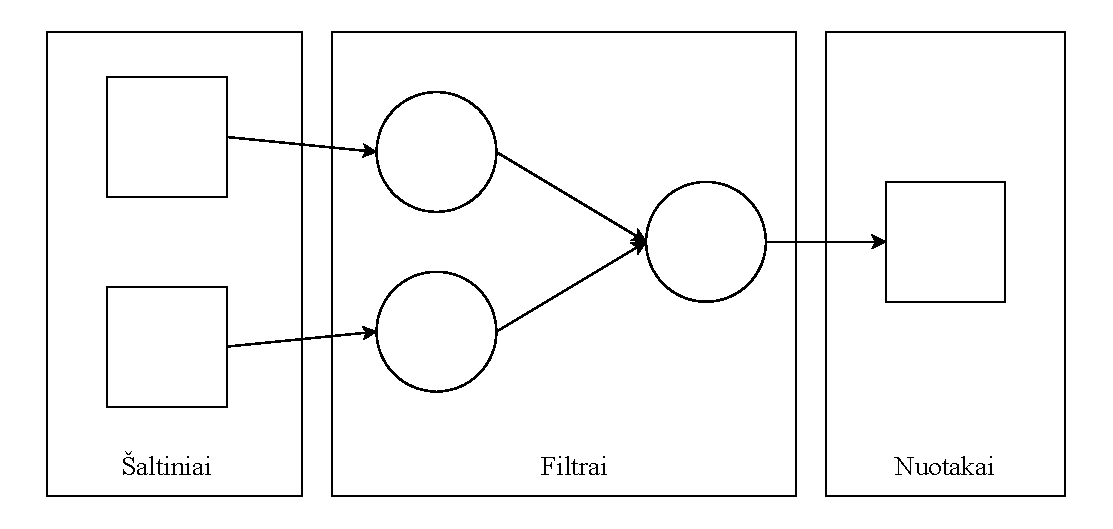
\includegraphics[width=15cm]{img/Srautinio apdorojimo sistema.pdf}
    \caption{Srautinio apdorojimo sistemos pavyzdys}
    \label{srautinio-apdorojimo-sistema}
\end{figure} 
Srautinio apdorojimo sistemos literatūroje yra vaizduojamos orientuotais grafikais (\ref{srautinio-apdorojimo-sistema} pav.). Srautinio apdorojimo sistemos skiriasi nuo reliacinių modelio šiais aspektais \cite{babcock2002models}: 
\begin{itemize}
    \item Duomenys į sistemą patenka tinklu, o ne iš fizinių talpyklų.
    \item Duomenų patekimo tvarka negali būti kontroliuojama.
    \item Duomenų kiekis yra neapibrėžtas.
    \item Duomenys apdoroti srautinio apdorojimo sistema yra pašalinami arba archyvuojami, t.y. juos pasiekti yra sunku. 
\end{itemize}
\subsubsection{Duomenų vykdymas}
Srautinio apdorojimo sistemų veikimui reikalingas srautinio apdorojimo variklis (angl. stream processing engine). Šie varikliai yra skirti srautinio apdorojimo sistemų vykdymui, dislokavimui, plečiamumo (angl. scaling) užtikrinimui ir gedimų tolerancijai (angl. fault–tolerance) \cite{zhao2017taxonomy}. Populiariųjų srautinio apdorojimo variklių pavyzdžiai: „Apache Storm“, „Apache Heron“, „Apache Spark“, „Apache Samza“ ir t.t \cite{roger2019comprehensive}. 
Duomenų vykdymas gali būti išskaidytas į tris elementus \cite{zhao2017taxonomy}: 
\begin{itemize}
    \item Planavimas (angl. scheduling) – duomenų apdorojimo užduočių planavimas daro įtaką bendram srautinio apdorojimo sistemos veikimui \cite{falt2011task}. Pavyzdžiui, „Apache Samza“ naudoja „Apache YARN“ resursų valdymo sistemą, kuri turi planavimo posistemę, kuri skirsto resursus \cite{noghabi2017samza} 
    \item Plečiamumas (angl. scalability) – apibrėžia daug apdorojimo branduolių turinčios sistemos gebėjimą apdoroti didėjanti kiekį užduočių ir galimybę didinti pačią sistemą, kad ji galėtų susidoroti su didėjančiu kiekiu duomenų \cite{bondi2000characteristics}. Srautinio apdorojimo varikliai turi užtikrinti srautinio apdorojimo sistemų plečiamumą \cite{stonebraker20058}.    
    \item Išskirstytas skaičiavimas (angl. Distributed computation) – tarpusavyje nesusiję skaičiavimo elementai turi naudotojui atrodyti kaip viena darni sistemą \cite{tanenbaum2007distributed}. Srautinio apdorojimo varikliai turi užtikrinti darbų paskirstymą ir skaičiavimo įrenginių koordinaciją, kad kuo daugiau duomenų būtų apdorojami vienu metu \cite{zhao2017taxonomy}.
\end{itemize}
Srautinio apdorojimo sistemos turi viena pagrindinį elementą – srauto procesorių (angl. stream processor), kuris apibrėžia sistemos elementus, aprašo kaip šie sistemos elementai sujungti ir pateikia nustatymus elementams \cite{zhao2017taxonomy}. Pavyzdžiui, „Apache Storm“ šis elementas vadinimas „topology“, kuris yra užrašomas Java kalba, naudojant „Apache Storm“ pateiktą biblioteką \cite{iqbal2015big}.
\subsubsection{Duomenų priėmimas}
Į srautinio apdorojimo sistemą duomenys patenka per šaltinius, kurie šiuos duomenis perduoda tolimesniems elementams. Dažniausiai duomenis perduodami į sistemą naudojant žinučių eiles (angl. message queues), nes jos turi buferi, kuris leidžia mažinti greičių skirtumus tarp duomenų gavimo ir duomenų apdorojimo ir žinučių eilių brokeriai gali išfiltruoti duomenis ir nukreipti juos į tinkamus šaltinius \cite{kamburugamuve2016survey}. Tačiau šaltiniai turi turėti galimybę rinkti išsaugotus duomenis ir priimti ateinančius naujus duomenis \cite{stonebraker20058}, todėl, nors ir šaltiniai dažniausiai skirti priimti srautinius duomenis, jie turi taip pat gebėti naudoti duomenis iš talpyklų \cite{zhao2017taxonomy}. 

\subsection{Srautinio apdorojimo sistemų matavimas}
Svarbiausias srautinio apdorojimo sistemų reikalavimas – duomenų apdorojimas ir rezultatų grąžinimas negali turėti atsilikimo – didelių apimčių srautiniai duomenys turi būti apdorojami taip pat greitai kaip jie ateiną \cite{stonebraker20058}. 

\subsubsection{Srautinio apdorojimo sistemų metrikos}
Pagrindinės kitų autorių naudojamos metrikos:
\begin{itemize}
    \item Pralaidumas (angl. Throughput) – per tam tikrą laiko tarpą apdorojamų įvykių kiekis.
    \item Vėlinimas (angl. Latency) – laiko intervalas nuo apdorojimo arba įvykio pradžios iki apdorojimo pabaigos.
\end{itemize}
Vėlinimas ir pralaidumas dažniausiai nepriklauso vienas nuo kito – sistemos, apdorojančios srautus mikro–paketais, turi didesnį pralaidumą, tačiau atsiranda papildomas vėlinimas, kol laukiama duomenų paketo apdorojimo pradžios \cite{Karimov2018BenchmarkingDS}. \par

\cite{stonebraker20058} straipsnyje minima, jog srautinio apdorojimo sistemos naudotojas turi išbandyti savo sistemą su tiksliniu darbo krūviu ir išmatuoti jos pralaidumą ir vėlinimą prieš naudodamas ją realiomis sąlygomis. \cite{Karimov2018BenchmarkingDS} lygina srautinio apdorojimo variklius ir matavimui naudoja vėlinimą, kurį išskaido į įvykio vėlinimą (angl. event–time latency) – laiko intervalas nuo įvykio laiko iki rezultato gavimo iš srautinio apdorojimo sistemos ir apdorojimo vėlinimą (angl. processing–time latency) – laiko intervalas nuo duomens patekimo į srautinio apdorojimo sistemą iki rezultato grąžinimo. Autoriai atlieka šį skaidymą, nes sistemų vertinime dažnai ignoruojamas įvykio laikas ir rezultatuose gaunamas daug mažesnis vėlinimas, nei tikras. Taip pat autoriai išskiria darnų pralaidumą (angl. sustainable throughput) – didžiausia apkrova įvykių, kurią sistema gali apdoroti be pastoviai augančio įvykio vėlinimo, todėl savo eksperimentuose autoriai užtikrina, kad duomenų generavimo greitis atitiktų sistemos darnų pralaidumą. Kad sužinoti darnų pralaidumą sistemos autoriai pradžioje leidžia labai didelį srautą duomenų ir mažina jį kol sistemos apdorojimas susivienodina su generavimo greičiais. Visus vėlinimo rezultatus autoriai pateikia maksimalaus pralaidumo apdorojimo ir 90\% pralaidumo apdorojimo vidurkiais, minimumais, maksimumais ir kvantiliais (90, 95, 99). \cite{hirzel2014catalog} autoriai nagrinėja srautiniam apdorojimui galimas optimizacijas ir matavimui naudoja normalizuotą pralaidumą (naudojamas vienetas kaip vidurkis), kadangi tai leidžia lengviau palyginti santykinę greitaveiką. Taip pat, \cite{hirzel2014catalog} pastebi, nors ir yra daug metrikų, kuriomis galima matuoti optimizacijos efektus: pralaidumas, vėlinimas, paslaugos kokybė (angl. quality of service), energijos ir tinklo panaudojimas, tačiau dažniausiai pagerinus pralaidumą pagerėja ir visos kitos metrikos. \cite{Qian2016Benchmarking} srautinių apdorojimo sistemų matavimui naudoja pralaidumą (skaičiuojama baitais per sekundę) ir vėlinimą, kaip vidurkį nuo duomens patekimo į sistemą iki apdorojimo pabaigos. Taip pat, kadangi autoriai lyginą srautinio apdorojimo variklius, jie įveda metriką gedimų toleravimo (angl. fault tolerance) matavimui – išjungiamas tam tikras kiekis elementų ir matuojamas pralaidumas ir vėlinimas. \cite{zhang2020heron} palyginimui naudoja sistemos įvykdymo vėlinimą (angl. system completion latency), kuris rodo vidutinį laiko tarpą per kurį duomuo nukeliauja nuo šaltinio iki sistemos galutinio taško. Autoriai skaičiavo vidutinį laiką 5 sekundžių intervalais. Taip pat autoriai matavimui naudoja kiekvienos instancijos (angl. instance) CPU apkrovą, kiekvieno darbinio mazgo (angl. worker node) CPU apkrovą ir apkrovą tarp instancijų/mazgų, kadangi \cite{zhang2020heron} užduotis – patobulinti esamą planavimo posistemę. \cite{dhalion} matavimui naudoja pralaidumą per minutę. \cite{vaquero2018autotuning} tyria labai panašią problemą – srautinių apdorojimo sistemų balansavimą taikant skatinamąjį mokymą ir matavimui naudoja vėlinimo 99 kvantilį. \cite{Chintapalli2016Benchmarking} srautinio apdorojimo variklių vertinimo tyrimui naudoja vėlinimą.

\begin{table}[H]
    \centering
    \caption{Metrikos naudojamos tiriant srautinio apdorojimo sistemų greitaveiką}
    \begin{tabular}{|l|l|l|}
    \hline
    Šaltinis                 & Vėlinimas                        & Pralaidumas                    \\ \hline
    \cite{stonebraker20058}  & Taip                             & Taip                           \\ \hline
    \cite{Karimov2018BenchmarkingDS} & Taip                     & Taip                           \\ \hline
    \cite{hirzel2014catalog} & Ne                               & Taip                           \\ \hline
    \cite{Qian2016Benchmarking} & Taip                          & Taip                           \\ \hline
    \cite{zhang2020heron}    & Taip                             & Ne                             \\ \hline
    \cite{dhalion}           & Ne                               & Taip                           \\ \hline
    \cite{vaquero2018autotuning} & Taip                         & Ne                             \\ \hline
    \cite{Chintapalli2016Benchmarking} & Taip                   & Ne                             \\ \hline
    \end{tabular}
\label{metrikos}
\end{table}

Pagal literatūros analizę (\ref{metrikos} len.) matome, kad dauguma autorių renkasi vertinti tik pagal vieną metriką ir dažniau matavimui naudojamas vėlinimas. Taip pat \cite{vaquero2018autotuning}, naudojantis skatinamąjį mokymą, matavimui naudoja vėlinimą ir \cite{Chintapalli2016Benchmarking} straipsnis, kuris siūlo srautinio apdorojimo sistemų vertinimo sprendimą, naudoja vėlinimą. Todėl magistro darbe matavimui bus naudojamas vėlinimas.   

\subsubsection{Srautinio apdorojimo sistemos pobūdis}

Srautinio apdorojimo sistemos gali turėti skirtingą elementų išsidėstymą ir nuo to priklausys jų greitaveiką. \cite{Karimov2018BenchmarkingDS} matavimui naudoja du filtrus – agregavimo, kuris skaičiuoja visus pirkimus ir jungimo (angl. join), kuris skaičiuoja duomenis pagal tam tikrą bendrą rodiklį iš abiejų duomenų srautų. \cite{Qian2016Benchmarking} srautinio apdorojimo variklių palyginimui naudoja septynis skirtingus uždavinius. Vienas iš jų yra WordCount uždavinys, kuris yra plačiai priimtas kaip didelių duomenų apdorojimo sistemos matavimo standartas \cite{huang2010hibench}. Šis uždavinys susidaro iš dviejų filtrų: pirmas išskaido teksto eilutę į žodžius, o antras agreguoja kiekvieno žodžio bendrą skaitiklį ir atnaujina bendrą žodžių panaudojimo dažnio rezultatą, kuriame raktas – žodis, o reikšmė skaičius, kuris rodo kiek kartojosi šis žodis (\ref{wordcount} pav.). 
\begin{figure}[H]
    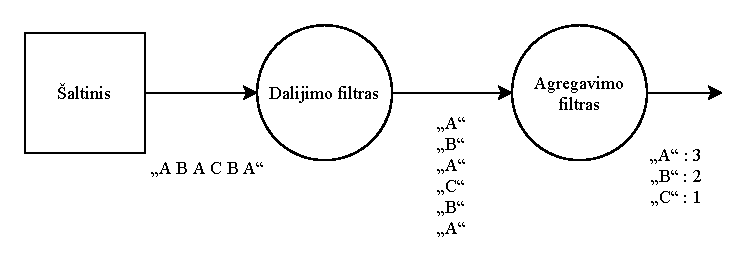
\includegraphics[width=15cm]{img/wordcount.pdf}
    \caption{WordCount sistemos pavyzdys}
    \label{wordcount}
\end{figure} 
\cite{zhang2020heron} matavimui naudoja WordCount sistemą, kuri yra paprastesnė, nei pavaizduota \ref{wordcount} paveikslėlyje, nes šaltinis generuoja ir siunčia tik po vieną žodį ir todėl yra tik agregavimo filtras. Taip pat autoriai  naudoja SentenceWordCount sistemą, kuri yra identiška \ref{wordcount} paveikslėlyje pavaizduotai sistemai. Bei autoriai sukūrė FileWordCount sistemą, kuri atlieka tą patį kaip ir SentenceWordCount, tačiau šaltinis negeneruoja žodžius, o skaito iš tekstinio dokumento ir taip pat naudoja egzistuojančią Yahoo srautinio apdorojimo vertinimą (angl. benchmarking) \cite{Chintapalli2016Benchmarking}. \cite{dhalion} autoriai naudoja WordCount eksperimentui. \cite{vaquero2018autotuning} eksperimentams naudoja Yahoo srautinio apdorojimo variklių vertinimą \cite{Chintapalli2016Benchmarking} ir taip pat atlieka bandymus su realiais daiktų interneto (angl. internet of things) įmonės duomenimis. \cite{Chintapalli2016Benchmarking} apibrėžia srautinio apdorojimo sistemą skirtingu srautinio apdorojimo variklių vertinimui. Pateikiama sistema analizuoja reklamas pagal kampaniją ir matomumą ir rezultatus deda į Redis duomenų bazę. Sistema sukurta taip, kad aprėptų visas srautinio apdorojimo sistemos savybes (\ref{yahoo} pav.).
\begin{figure}[H]
    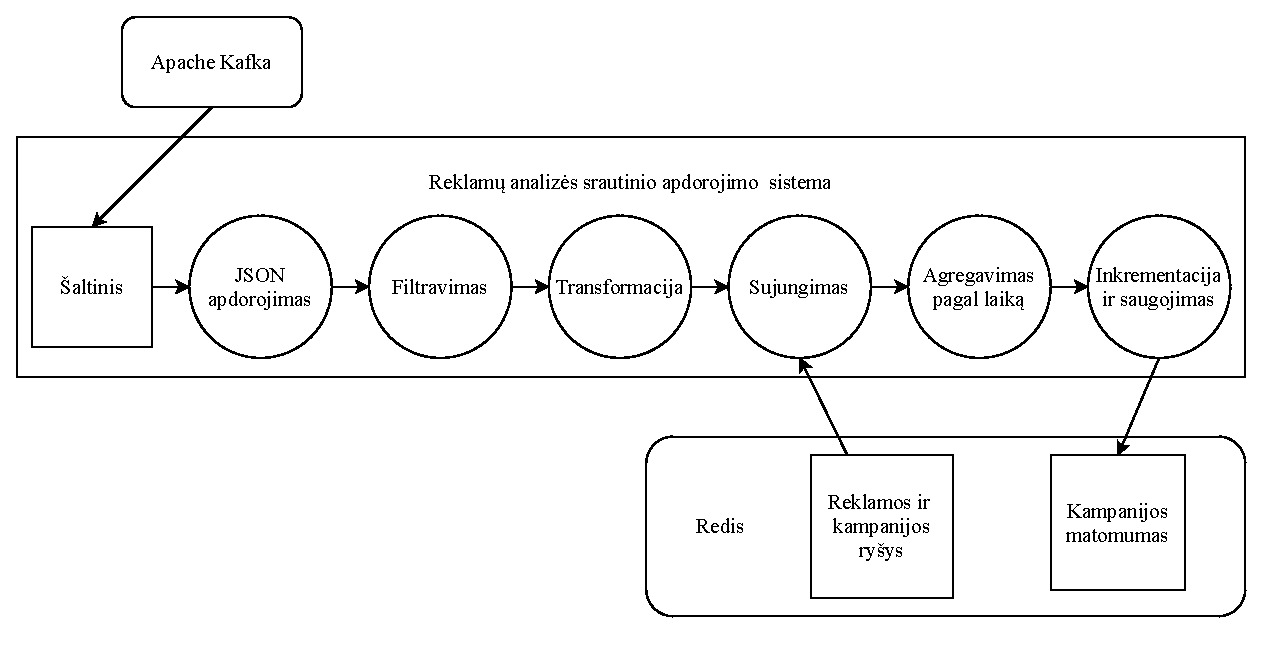
\includegraphics[width=15cm]{img/yahoo.pdf}
    \caption{Reklamų analizės sistema \cite{Chintapalli2016Benchmarking}}
    \label{yahoo}
\end{figure} 

Straipsniai (\cite{Qian2016Benchmarking, huang2010hibench, dhalion}) naudoja WordCount (\ref{wordcount} pav.), o \cite{Chintapalli2016Benchmarking, vaquero2018autotuning} naudoja Reklamų analizės srautinę apdorojimo sistemą (\ref{yahoo} pav.). Magistro darbe ketinama atlikti tyrimus su Reklamų analizės sistema, kadangi ši sistema sukurta srautinių apdorojimo variklių vertinimui ir su WordCount srautinio apdorojimo sistemą, kuri neturi pašalinių elementų sistemoje, kadangi Reklamų analizės sistema naudoja „Apache Kafka“, „Redis“ vertinimui.    

\subsubsection{Srautinio apdorojimo sistemų matavimo duomenys}

Vertinant sistemų greitaveiką reikia atsižvelgti ir į testavimui naudojamus duomenis. \cite{Karimov2018BenchmarkingDS} naudoja žaidimų kūrimo įmonės Rovio duomenis ir naudoja du duomenų srautus – pirkimo srautas, kuriame siunčiami kortežai (angl. tuples) sudaryti iš nupirktos valiutos kiekio, laiko ir naudotojo, kuris ją nupirko ir reklamų srautas, kuris siunčia valiutos reklamas tam tikru laiku. Šiame sprendime duomenis generuojami naudojant normalizuotą paskirstymą ant raktinio lauko. \cite{Qian2016Benchmarking} naudoja tekstinius duomenis iš AOL paieškos variklio ir apdoroja juos pagal pasirinktus uždavinius. \cite{zhang2020heron} matavimui naudoja šaltinių generuojamą tekstą, kadangi lyginamas tas pats srautinio apdorojimo variklis tik su patobulinta planavimo posisteme ir naudoja iš anksto sugeneruotą tekstą patalpintą į tekstinį dokumentą. \cite{Chintapalli2016Benchmarking} aprašo sistemą, kuri daro skirtingų srautinio apdorojimo variklių vertinimą. Šiam vertinimui naudojami duomenys simuliuojantys reklamas ir reklamų kampanijas. Autoriai naudoja savo duomenų generatorių. 
Magistro darbe ketinama naudoti \cite{Chintapalli2016Benchmarking} pateikiamą Reklamos analizės sistemos duomenų generatorių, o WordCount srautinės apdorojimo sistemos tyrimui ketinama naudoti WordCount šaltinio generuojamus duomenis.

\subsection{Srautinio apdorojimo sistemų derinimas}
Sistemų greitaveika yra tiesiogiai susijusi su konfigūravimo parametrais, kurie valdo tokius aspektus kaip: atminties valdymas, gijų skaičius, planavimas, resursų valdymas \cite{lu2019speedup}. Taip pat, neteisingi nustatymai turi nuostolingus efektus sistemos greitaveikai ir stabilumui \cite{herodotou2011starfish}. 

\cite{herodotou2020survey} išskiria 3 pagrindinius automatinio derinimo iššūkius:
\begin{enumerate}
    \item Didelė ir sudėtinga parametrų erdvė – „Apache Spark“ ir „Apache Storm“ turi virš 150 konfigūruojamų parametrų \cite{Bilal2017Towards, petridis2016spark}. Taip pat, nustatymų reikšmės, kurios tinka vienam uždaviniui, gali turėti neigiamos įtakos kitam \cite{herodotou2011starfish, Pooyan2016Uncertainty}.
    \item Sistemų mastas ir sudėtingumas – Sistemų administratoriai turi gebėti konfigūruoti didelius kiekius skaičiavimo mazgų, kurie gali turėti skirtingus CPU, atminties, tinklo tipus \cite{herodotou2020survey}.
    \item Pradinių duomenų statistikos trūkumas – įvedimo duomenys srautinėse apdorojimo sistemose yra realus srautai, kurie stipriai varijuoja savo apimtimi \cite{Dayarathna2018Recent}.
\end{enumerate}  

\cite{Trotter2017Into} nagrinėjantis tinkamos konfigūracijos radimą naudojant genetinius algoritmus „Apache Storm“ srautinio apdorojimo sistemoms nustatė, jog lygiagretumo laipsnis labiausiai daro įtaką srautinio apdorojimo sistemų greitaveikai. „Apache Heron“ srautinio apdorojimo variklis, kuris yra „Apache Storm“ su patobulinimais \cite{twitterHeron}, pateikia naują būdą kontroliuoti srautą – priešslėgis (angl. backpressure), kuris leidžia filtrui sulėtinti prieš jį einantį elementą, kas leidžia sumažinti vėlinimą ir taip pat gali būti naudojamas kaip greitaveikos praradimo indikatorius \cite{bansal2018trevor}.
Taip pat \cite{bansal2018trevor} nagrinėja „Apache Heron“ automatinį konfigūravimą naudojant iš anksto aprašytas taisykles. 

\section{Mašininis mokymasis}

\subsection{Mašininis mokymasis srautinio apdorojimo sistemų derinimui}

\cite{herodotou2020survey} aprašo skirtingus sprendimus automatiniam konfigūravimui ir išskiria šiuos mašininio mokymosi privalumus:
\begin{itemize}
    \item Nebūtina suprasti sistemos, užduočių ir duomenų, kadangi naudojamas juodos dėžės (angl. black–box) principas.
    \item Mašininio mokymosi modelis pats save tobulina, ir yra vis tikslesnis kuo daugiau gauna duomenų. 
\end{itemize}
Šio straipsnio autoriai išskiria mašininio mokymosi iššūkius: 
\begin{itemize}
    \item Parametrų parinkimas – kadangi konfigūruojamų parametrų kiekis yra didelis \cite{Bilal2017Towards, petridis2016spark} ne visi iš jų vienodai daro įtaką greitaveikai, todėl pirma verta išsirinkti aktualiausius parametrus resursų valdymo, užduočių planavimo ir duomenų valdymo užduotims. Tam dažnai naudojama eksperto pagalba \cite{wang2016novel}, gidai arba eksperimentavimas. Tačiau galima naudoti mašininio mokymosi algoritmą koreliacijos nustatymui tarp parametrų ir greitaveikos \cite{vaquero2018autotuning, yang2012statistics}
    \item Mašininio mokymosi modelio pasirinkimas – kadangi yra nemažai skirtingų mašininio mokymosi metodų kurie tinka derinimo uždaviniui.
\end{itemize} 
Taip pat autoriai pateikia paketinio ir srautinio apdorojimo derinimą naudojant mašininį mokymąsi straipsnius (\ref{ml-in-stream} lentelėje pateikiami tik išrinkti srautinio apdorojimo pavyzdžiai).

\begin{table}[H]
    \centering
    \caption{Srautinių sistemų derinimo naudojant mašininį mokymąsi pavyzdžiai \cite{herodotou2020survey}}
    \begin{tabular}{|l|p{0.40\textwidth}|p{0.20\textwidth}|}
    \hline
    Šaltinis                                        & Įvesties savybės                                                                    & Mašininio mokymosi metodai                 \\ \hline
    Zacheilas et al. \cite{zacheilas2015elastic}    & Rinkinys kelių konfigūracijos parametrų                                             & Gaussian Processes                         \\ \hline
    Li et al. \cite{li2016performance}              & Atminties dydžiai ir branduolių ir gijų kiekis skirtingose stadijose                & Support Vector Regression                  \\ \hline
    Trotter et al. \cite{Trotter2017Into}           & Darbinių procesų kiekis, vykdytojų kiekis                                           & Genetic Algorithm, Bayesian Optimization   \\ \hline
    Trotter et al. \cite{trotter2019forecasting}    & Vykdytojai, šaltinių ir filtrų lygiagretumas, acker lygiagretumas                   & Genetic Algorithm, Support Vector Machines \\ \hline
    OrientStream \cite{wang2017automating}          & Įvairios duomenų, plano, filtrų ir klasterio lygio savybės                          & Ensemble/ Incremental ML                    \\ \hline
    Vaquero et al. \cite{vaquero2018autotuning}     & Parametrai ir metrikos parinkti faktorinės analizės (angl. factor analysis) pagalba & Reinforcement Learning                     \\ \hline
    \end{tabular}
    \label{ml-in-stream}
\end{table}

\subsection{Skatinamasis mokymasis srautiniam apdorojimui}

\cite{vaquero2018autotuning} nagrinėja srautinių sistemų derinimą naudojant skatinamąjį mokymąsi. Autoriai pradžioje pasirenka Lasso path analysis algoritmą, kurio pagalba atlieka parametrų atranka, kad išrinktų svarbiausius parametrus pasirinktos metrikos valdymui. Konfigūracijos valdymui pasirinktas modifikuotas REINFORCE algoritmas. Atliktas eksperimentas su „Apache Spark“, kuris rodo 60–70\% sumažintą vėlinimą.

\cite{ni2019generalizable} nagrinėja resursų valdymo problemą srautinio apdorojimo sistemose ir siūlo sprendimą naudojanti skatinamąjį mokymą, kuris daro optimizacijas pagal srautinės apdorojimo sistemos grafus. Eksperimentas atliekamas naudojant REINFORCE \cite{williams1992simple} algoritmą su Adam optimizacijos funkcija \cite{kingma2014adam} ir atliekamas eksperimentas naudojant tyrimui parašytą srautinio apdorojimo variklį ir sistemas. 

\cite{Li2018Model} nagrinėja planavimo problemos (apkrovos paskirstymas darbiniams elementams) sprendimą naudojant skatinamąjį mokymąsi. Autoriai siūlo naudoti Actor−Critic {lillicrap2015continuous} metodą naudojant Deep Q Learning  \cite{mnih2015human} tinklą kaip Actor ir bet kokį gilųjį neuroninį tinklą kaip Critic. Autorių rezultatai rodo 45\% greitaveikos padidėjimą lyginant su integruota „Apache Storm“ planavimo posisteme. 

\cite{Russo2019Reinforcement} nagrinėja srautinių sistemų dislokavimą naudojant skatinamąjį mokymą. Sprendžiama problema dislokavimo valdymo su skirtingais skaičiavimo mazgų tipais. Naudojamas Q Learning algoritmas su įvairioms modifikacijom (kombinuojama su tiksliais modeliais). Autoriai matuoja dislokavimo tikslumą ir konvergavimo greitį. 

\begin{table}[H]
    \centering
    \caption{Skatinamojo mokymosi naudojimas}
    \begin{tabular}{|l|l|}
    \hline
    Šaltinis                         & Skatinamojo mokymosi algoritmas    \\ \hline
    \cite{vaquero2018autotuning}     & Adaptuotas REINFORCE \cite{williams1992simple}        \\ \hline
    \cite{ni2019generalizable}       & REINFORCE \cite{williams1992simple}  su Adam optimizacijos funkcija \cite{kingma2014adam}     \\ \hline
    \cite{Li2018Model}               & Deep Q Learning \cite{mnih2015human} ir Actor−Critic \cite{lillicrap2015continuous} \\ \hline
    \cite{Russo2019Reinforcement}    & Q–learning \cite{mnih2015human} su papildomomis funkcijomis \\ \hline
    \end{tabular}
    \label{ml-usage}
\end{table}

\section{Srautinės duomenų apdorojimo sistemos, valdomos mašininiu mokymusi, modelis}

Tyrime nagrinėjamas srautinės sistemos, balansuojamos mašininių mokymų, modelis (\ref{dataflow} pav.) susidaro iš trijų pagrindinių elementų: srautinio duomenų apdorojimo sistemos, srautinio duomenų apdorojimo platformos ir valdymo sistemos. 
\subsection{Modelis}
\begin{figure}[H]
    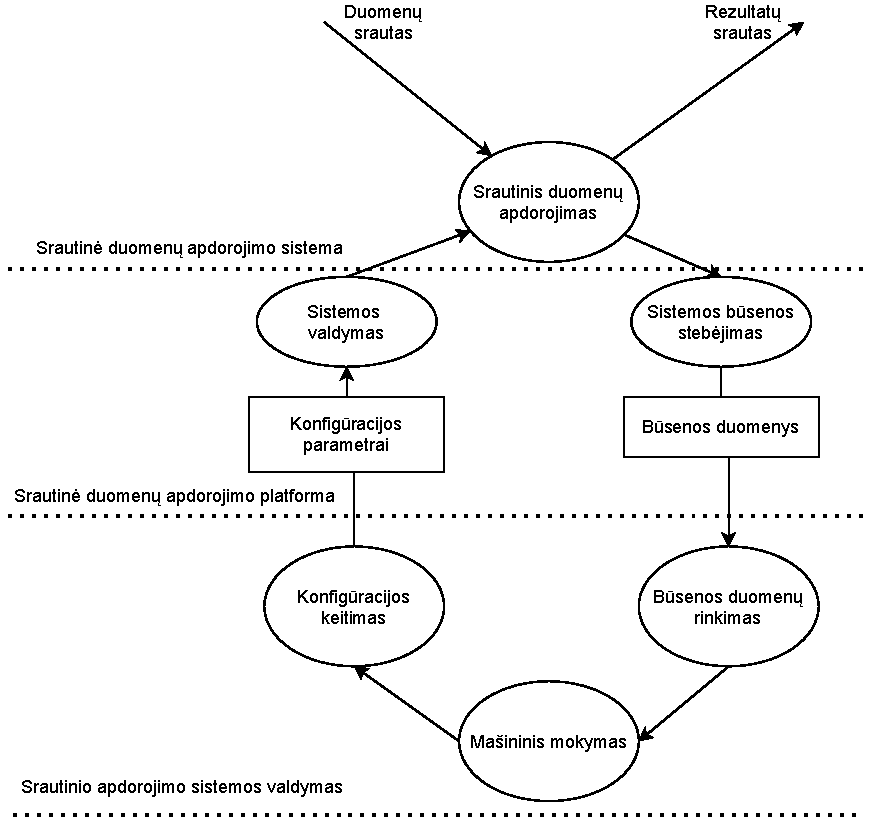
\includegraphics[width=15cm]{img/DataFlow.pdf}
    \caption{Srautinės apdorojimo sistemos modelis}
    \label{dataflow}
\end{figure} 
Srautinės duomenų apdorojimo sistemą sudaro šie elementai:
\begin{itemize}
    \item Duomenų srautas – duomenys patenkantys į srautinio apdorojimo sistemą nepertraukiamu srautu, iš anksto nežinomu greičiu ir nekontroliuojamu kiekiu.
    \item Srautinis duomenų apdorojimas – srautinio duomenų apdorojimo sistema, atliekanti skaičiavimus su duomenimis ateinančiais iš duomenų srauto. Tyrime naudojamos Heron srautinio apdorojimo sistemos pasižymi individualiais skaičiavimo komponentais, kurie skaičiuoja kiekvieną patenkantį duomenį ir yra parašyti užtikrinant lygiagretumą komponento lygyje.
    \item Rezultatų srautas – duomenys apdoroti srautinio duomenų apdorojimo sistemos ir perduoti iš paskutinio skaičiavimo komponento į kitas sistemas.
\end{itemize}
Srautinio apdorojimo sistemų platforma turi šiuos elementus:
\begin{itemize}
    \item Srautinį duomenų apdorojimą.
    \item Sistemos būsenos stebėjimą – srautinio apdorojimo platformos sistema renkanti srautinio apdorojimo sistemų veikimo metrikas ir šias metrikas atskleidžianti į išorę. Tyrime naudojama Heron platforma metrikas pateikia kiekvienam skaičiavimo komponentui individualiai per HTTP protokolą arba į naudotojo pateiktą metrikų surinkimo sistemą.
    \item Būsenos duomenys – tai metrikos vaizduojančios kiekvienos srautinio apdorojimo sistemos skaičiavimo komponentų  veikimo rodiklius, tokius kaip vėlinimas, pralaidumas, apkrovos ir t.t.
    \item Konfigūracijos parametrai – tai konfigūracijos rinkinys kurį apibrėžia srautinio apdorojimo platforma. Šie konfigūracijos parametrai nurodo srautinės apdorojimo sistemos veikimą ir taip pat gali apibrėžti parametrus skirtus individualiems skaičiavimo komponentams. Tyrime naudojama Heron platforma apibrėžia ir valdo visus srautinės apdorojimo sistemos konfigūracijos parametrus.
    \item Sistemos valdymas – konfigūracijos parametrų pateikimas į srautinio apdorojimo platformą. Šie konfigūracijos parametrai nurodo srautinės apdorojimo sistemos ir jos skaičiavimo komponentų veikimą. Tyrime naudojama Heron platformą leidžia pateikti konfigūracijos parametrus per komandinę eilutę. Pateikus konfigūraciją platforma sustabdo srautinę apdorojimo sistemą, atnaujina jos konfigūraciją ir paleidžia sistemą iš naujo. Kai sistema sustabdoma, taip pat nustojama ir skaityti duomenis iš duomenų srauto, o paleidus sistemą duomenys skaitomi toliau.
\end{itemize}
Srautinio apdorojimo sistemos valdymo elementai susidaro iš:
\begin{itemize}
    \item Būsenos duomenų rinkimo – tai sistema renkanti duomenis apie srautinės apdorojimo sistemos būseną iš srautinės apdorojimo platformos. Ši sistema atsakinga už aktualių metrikų surinkimą, kurios naudojamos suformuoti vaizdą apie srautinio duomenų apdorojimo sistemos būseną.
    \item Mašininio mokymosi – sistema, kurį gauna srautinės apdorojimo sistemos būsenos duomenis ir pagal tai apskaičiuoja naujas konfigūracijos parametrų reikšmes. Tyrime naudojamas skatinamasis mašininis mokymasis, kuris nuolatos bando gerina sistemos būseną apskaičiuojant konfigūracijos parametrų pokyčius ir mokosi iš anksčiau padarytų sprendimų.
    \item Konfigūracijos keitimo – sistema priimanti atnaujintus konfigūracijos parametrus ir pateikianti juos į srautinio apdorojimo platformą. 
\end{itemize}

Visumoje \ref{dataflow} paveikslėlis apibrėžia duomenų judėjimą srautinio duomenų apdorojimo sistemos valdymo modelyje. Srautinio apdorojimo sistema yra pagrindinis elementas atsakingas už patį duomenų apdorojimą ir veikia nepriklausomai nuo kitų elementų modelyje. Srautinio apdorojimo platforma talpina ir palaiko srautinio apdorojimo sistemas, taip pat suteikia prieiga gauti informaciją apie srautinio apdorojimo sistemų būseną bei suteikia galimybę valdyti srautinio apdorojimo sistemas. Srautinio apdorojimo sistemų valdymo elementai atsakingi už srautinės apdorojimo sistemos konfigūracijos keitimą pagal surinktus būsenos duomenis.

\subsection{Keičiami konfigūracijos parametrai}

Norint koreguoti konfigūracijos parametrus reikia siųsti atnaujinimo komandą į Heron komandinės eilutės įrankį (toliau Heron CLI). Pateikus konfigūracijos parametrus Heron platformą perkrauna srautinio apdorojimo sistemą su naujais parametrais. 
Vienas iš pagrindinių srautinės apdorojimo sistemos konfigūracijos parametrų - skaičiavimo komponentų lygiagretumas, kuris nurodo kiek paleidžiama tam tikro komponento instancijų. Taip pat tai yra vienintelis keičiamas konfigūracijos elementas, kuris priklauso nuo valdomos srautinio apdorojimo sistemos sudėties.

Visi kiti konfigūravimo parametrai\cite{configDocument}, kurie taip pat yra keičiami balansavimo metu pateikti \ref{param–table} lentelėje:

\begin{longtable}{|p{0.59\linewidth}|p{0.41\linewidth}|}
    \caption{Keičiami konfigūracijos parametrai}
    \label{param–table}\\
    \hline
    \rowcolor[HTML]{C0C0C0} 
    Parametras                                              & Paaiškinimas                                                                                 \\ \hline
    \endfirsthead
    %
    \endhead
    %
    component–parallelism=[skaičiavimo komponento pavadinimas]            & Tam tikro skaičiavimo komponento lygiagretumas                                 \\ \hline
    heron.instance.tuning.expected.bolt.read.queue.size                   & Numatomas skaitomos eilės dydis Bolt tipo komponentuose                        \\ \hline
    heron.instance.tuning.expected.bolt.write.queue.size                  & Numatomas rašomos eilės dydis Bolt tipo komponentuose                          \\ \hline
    heron.instance.tuning.expected.spout.read.queue.size                  & Numatomas skaitomos eilės dydis Spout tipo komponentuose                       \\ \hline
    heron.instance.tuning.expected.spout.write.queue.size                 & Numatomas rašomos eilės dydis Spout tipo komponentuose                         \\ \hline
    heron.instance.set.data.tuple.capacity                                & Didžiausias kiekis kortežų sugrupuotu vienoje žinutėje                        \\ \hline
    heron.instance.emit.batch.time.ms                                     & Didžiausias laikas Spout tipo komponentui išsiųsti gautą kortežą               \\ \hline
    heron.instance.emit.batch.size.bytes                                  & Didžiausias partijos dydis Spout tipo komponentui išsiųsti gautą kortežą       \\ \hline
    heron.instance.execute.batch.time.ms                                  & Didžiausias laikas Bolt tipo komponentui apdoroti gautą kortežą                \\ \hline
    heron.instance.execute.batch.size.bytes                               & Didžiausias partijos dydis Bolt tipo komponentui apdoroti gautą kortežą        \\ \hline
    heron.instance.internal.bolt.read.queue.capacity                      & Skaitomos eilės dydis Bolt komponentams                                        \\ \hline
    heron.instance.internal.bolt.write.queue.capacity                     & Rašomos eilės dydis Bolt komponentams                                          \\ \hline
    heron.instance.internal.spout.read.queue.capacity                     & Skaitomos eilės dydis Spout komponentams                                       \\ \hline
    heron.instance.internal.spout.write.queue.capacity                    & Rašomos eilės dydis Spout komponentams                                         \\ \hline
    heron.api.config.topology\_container\_max\_ram\_hint                  & Daugiausiai operatyvios atminties kiekio konteineriui išskyrimo užuomina       \\ \hline
    heron.api.config.topology\_container\_max\_cpu\_hint                  & Daugiausiai procesoriaus pajėgumo konteineriui išskyrimo užuomina              \\ \hline
    heron.api.config.topology\_container\_max\_disk\_hint                 & Daugiausiai kietojo disko atminties kiekio konteineriui išskyrimo užuomina    \\ \hline
    heron.api.config.topology\_container\_padding\_percentage             & Užuominų galimą paklaidą                                                       \\ \hline
\end{longtable}

\subsection{Naudojamos metrikos}
Metrikos iš Heron srautinio apdorojimo sistemų gali būti pasiektos keliais skirtingais būdais: darant užklausą į Heron API, skaitant iš tekstinio failo, kurį pildo Heron platformą arba naudojant savo sukurtą metrikų skaitymo priedą, kuris pateikiamas į Heron platformą prieš ją paleidžiant. Visos metrikos yra saugomos srautinio apdorojimo sistemos kiekvienam skaičiavimo komponentui. 

\ref{metrics–table} lentelėje aprašytos metrikos yra standartinės visiems Heron srautinio apdorojimo sistemos komponentams ir grąžinamos iš Heron per Heron API \cite{heronTracker}. Šios metrikos ir bus perduodamos į mašininio mokymosi algoritmą kaip aplinkos būsenos apibūdinimas.

\begin{longtable}{|p{0.5\linewidth}|p{0.4\linewidth}|}
    \caption{Naudojamos metrikos}
    \label{metrics–table}\\
    \hline
    \rowcolor[HTML]{C0C0C0} 
    Metriką                                  & Paaiškinimas            \\ \hline
    \endfirsthead
    %
    \endhead
    %
    \_\_emit–count (toliau išsiųstas kiekis)                           & Išsiųstų kortežų kiekis                    \\ \hline
    \_\_execute–count  (toliau apdorotas kiekis)                       & Apdorotų kortežų kiekis Bolt komponentuose \\ \hline
    \_\_execute–latency  (toliau vidutinis apdorojimo vėlinimas)       & Vidutinė trukmė Bolt komponentui apdoroti kortežą                                          \\ \hline
    \_\_jvm–process–cpu–load  (toliau procesoriaus apkrova)            & JVM apkrova procesoriui     \\ \hline
    \_\_jvm–memory–used–mb    (toliau naudojamas RAM)                  & JVM naudojama operatyvi atmintis       \\ \hline
    \_\_jvm–memory–mb–total     (toliau išskirtas RAM kiekis)          & JVM turima operatyvi atmintis    \\ \hline
    \_\_jvm–gc–collection–time–ms  (toliau vidutinė GC trukme)         & JWM šiukšlių surinkimo trukmė     \\ \hline
    \_\_time\_spent\_back\_pressure\_by\_compid  (toliau bendra priešslėgio trukmė)  & Kiek laiko komponentui buvo įjungtas priešslėgio režimas  \\ \hline
\end{longtable}

\subsection{Tikslo funkcija}

Srautinio apdorojimo sistemos valdymo tikslas – keičiant konfigūraciją, pasiekti didžiausią greitaveiką. Šiame tyrime greitaveika matuojama vėlinimu, tačiau tuo pačiu turi būti palaikomas sistemos stabilumas ir duomenų pralaidumas. Todėl pasirinkti konfigūracijos elementai su koeficientais, kurie nurodo tam tikros metrikos svarbą pasiekti greitaveikai. 

\begin{longtable}{|p{0.55\linewidth}|p{0.15\linewidth}|p{0.2\linewidth}|}
    \caption{Metrikų tikslai}
    \label{goal–table}\\
    \hline
    \rowcolor[HTML]{C0C0C0} 
    Metrika                         & Koeficientas & Tikslas          \\ \hline
    \endfirsthead
    %
    \endhead
    %
    Išsiųstas kiekis                & 2 & \(\infty\)  \\ \hline
    Apdorotas kiekis                & 2 & \(\infty\) \\ \hline
    Vidutinis apdorojimo vėlinimas  & 3 & 0    \\ \hline
    Naudojamas RAM                  & 1 & Išskirtas RAM – Naudojamas RAM = 0      \\ \hline
    Vidutinė GC trukmė              & 1 & 0    \\ \hline
    Bendra priešslėgio trukmė       & 2 & 0    \\ \hline
\end{longtable}

\ref{goal–table} lentelėje pateiktos metrikos, šių metrikų svarumo koeficientas ir jų tikslas. Metrikų koeficientas pasirinktas pagal tai, jog visų pirma yra optimizuojama turėti kuo mažesnį vėlinimą. 

\section{Balansavimo algoritmas}

\subsection{Srautinės architektūros sistemos konfigūracijos valdymo algoritmas}

Algoritmo tikslas – pagal esamą būseną ir esamą konfigūraciją apskaičiuoti naują konfigūraciją, kuri pagerintų srautinės apdorojimo sistemos greitaveiką. Algoritmo pagrindas yra pasirinkti skatinamojo mašininio mokymosi algoritmai Deep Q Network ir Soft Actor Critic.

Kad algoritmas galėtų apskaičiuoti naują konfigūraciją, jam yra paduodami šie duomenys:
\begin{itemize}
    \item Srautinio apdorojimo sistemos metrikos (\ref{metrics–table} lentelė)
    \item Srautinio apdorojimo sistemos pradinė konfigūracija (\ref{param–table-pract} lentelė).
    \item Konfigūruojamų parametrų sąrašas ir jų galimos reikšmės, aprašytos intervalu (pavyzdžiui \([512,4096]\)) arba tiksliais variantais (pavyzdžiui \([512, 1024, 2048, 4096]\)).
\end{itemize}
Duomenys, kurie paduodami balansavimo algoritmui, yra renkami pastoviai, neatsižvelgiant į pačio algoritmo veikimą.

Balansavimo algoritmas veikia ciklais visą srautinės apdorojimo sistemos veikimo laiką ir tarpas tarp ciklų turi būti pakankamai ilgas srautinio apdorojimo sistemai atsinaujinti su naujais konfigūracijos parametrais bei, kad surinktų duomenų kiekis būtų pakankamai svarūs pateikti mašininio mokymosi algoritmui. Balansavimo algoritmas, atlikęs skaičiavimus, grąžina naują konfigūracijos parametrų rinkinį ir laukia naujo ciklo pradžios. 

Balansavimui naudojami skatinamojo mašininio mokymosi algoritmai Deep Q network \cite{fan2020theoretical} ir Soft Actor Critic \cite{haarnoja2019soft} turi bendrus veikimo bruožus:
\begin{itemize}
    \item Jie yra laisvo nuo modelio (angl. model–free) tipo skatinamojo mokymosi algoritmai, tai yra - jie daro sprendimus pagal tai, ką išmoko veikimo metu ir negeneruoja bendro modelio. Tai aktualu mūsų atveju kadangi balansavimo algoritmas turi galėti prisitaikyti prie kintančių duomenų kiekio ir greičio bei kintančios aplinkos.
    \item Jie yra be strategijos (angl. off–policy) tipo, tai reiškia, kad jie mokosi atliekant skirtingus veiksmus, nebūtinai tuos, kurie buvo pasirinkti pagal dabartinę strategiją.
\end{itemize} 

Šie algoritmai buvo pasirinkti, nes skiriasi kaip apibrėžiamos veiksmų aibės – Deep Q Network galimų veiksmų aibę priima kaip rinkinį, o Soft Actor Critic kaip intervalą, todėl naudojant šiuos tinklus galimų konfigūruojamų parametrų aibė apsirašo skirtingai. 

\subsection{Srautinio duomenų apdorojimo aplinkos apibrėžimas balansavimui}

Balansavimui atlikti reikalingas tikslus apibrėžimas srautinio apdorojimo aplinkos, šis apibrėžimas susidaro iš: dabartinės srautinio apdorojimo sistemos būsenos, galimų veiksmų aibės ir žingsnio funkcijos, kuri atlieka veiksmą ir apskaičiuoja atpildą.

Srautinio apdorojimo sistemos dabartinė būsena – srautinio apdorojimo sistemos metrikos patalpintos masyve.

Srautinio apdorojimo sistemos balansavimo galimų veiksmų aibė – konfigūracijos parametrai, kuriuos algoritmas gali koreguoti ir jų reikšmių aibė. Kadangi Deep Q Network reikalauja diskrečių reikšmių, o Soft Actor Critic testinių reikšmių aibės, jos skirtingai paduodamos į balansavimo algoritmą, tačiau reikšmių ribos vienodos.
\begin{longtable}{|p{0.59\linewidth}|p{0.4\linewidth}|}
    \caption{Galimų veiksmų aibė}
    \label{param–table-pract}\\
    \hline
    \rowcolor[HTML]{C0C0C0} 
    Parametras     & Natūraliųjų reikšmių aibė       \\ \hline
    \endfirsthead
    %
    \endhead
    %
    component–parallelism=[skaičiavimo komponento pavadinimas]& \([1;10] * \text{Komponentų kiekis}\)\\ \hline
    heron.instance.tuning.expected.bolt.read.queue.size       & \([2;20]\) \\ \hline
    heron.instance.tuning.expected.bolt.write.queue.size      & \([2;20]\) \\ \hline
    heron.instance.tuning.expected.spout.read.queue.size      & \([128;512]\) \\ \hline
    heron.instance.tuning.expected.spout.write.queue.size     & \([2;20]\) \\ \hline
    heron.instance.set.data.tuple.capacity                    & \([64;512]\) \\ \hline
    heron.instance.emit.batch.time.ms                         & \([8;128]\) \\ \hline
    heron.instance.emit.batch.size.bytes                      & \([8192;65536]\) \\ \hline
    heron.instance.execute.batch.time.ms                      & \([8;128]\) \\ \hline
    heron.instance.execute.batch.size.bytes                   & \([8192;65536]\) \\ \hline
    heron.instance.internal.bolt.read.queue.capacity          & \([64;512]\) \\ \hline
    heron.instance.internal.bolt.write.queue.capacity         & \([64;512]\) \\ \hline
    heron.instance.internal.spout.read.queue.capacity         & \([512;4096]\) \\ \hline
    heron.instance.internal.spout.write.queue.capacity        & \([64;512]\) \\ \hline
    heron.api.config.topology\_container\_max\_ram\_hint      & \([256;2048]\) \\ \hline
    heron.api.config.topology\_container\_max\_cpu\_hint      & \([20;80]\) \\ \hline
    heron.api.config.topology\_container\_max\_disk\_hint     & \([8192;65536]\) \\ \hline
    heron.api.config.topology\_container\_padding\_percentage & \([0;20]\) \\ \hline
\end{longtable}

Srautinio apdorojimo sistemos balansavimo žingsnio funkcija:
\begin{itemize}
 \item Atliekamas veiksmas – naujos konfigūracijos įkėlimas ir nustatyto laiko laukimas, kad srautinio apdorojimo sistema pasiektų apkrovą.
 \item Atpildas – skaitinė reikšmė apskaičiuotą naudojant normalizuotas metrikas (apibrėžtas \ref{metrics–table} pav.) su koeficientais ir \ref{formula} formulę.
\end{itemize}
\begin{equation}
    \label{formula}
    \begin{gathered}
    \text{Atpildas} = 2*\text{Išsiųstas kiekis } + 2*\text{Apdorotas kiekis }  – \\ 
        3*\text{Vidutinis apdorojimo vėlinimas } – \text{ Naudojamas RAM }  – \\
          \text{Vidutinė GC trukme } – \:2*\text{Bendra priešslėgio trukmė} 
    \end{gathered}
\end{equation}
\subsection{Balansavimo algoritmo apmokymas}

Balansavimo algoritmo apmokymas vyks srautinio apdorojimo sistemos veikimo metu. Paleidus srautinę apdorojimo sistemą bus paleidžiamas ir balansavimo algoritmas. Tam, kad algoritmas turėtų pagrindą veiksmų pasirinkimui, algoritmo veikimo pradžioje konfigūracija bus pasirenkama atsitiktinai apibrėžtą ciklų kiekį ir renkami rezultatai mašininio tinklo apmokymui. Po šio ciklo algoritmas atliks sprendimus pagal patirtį. Deep Q Network ir Soft Actor Critic algoritmai naudoja pakartojimo buferio mokymosi optimizaciją, kai algoritmas mokosi ne iš paskutinio atlikto veiksmo, o iš atsitiktinai pasirinktos aibės, kurios elementai susidaro iš veiksmo, būsenos, atpildo ir naujos būsenos rinkinių. Pakartojimo buferio aibė saugoma viso mokymosi metu ir yra konfigūruojamas mokymosi metu pasirenkamos aibės dydis. 

\section{Eksperimento tyrimo planas}

\subsection{Tyrimo tikslas}

Šio tyrimo tikslas – įvertinti siūlomo balansavimo modelio ir pasirinkto optimizavimo algoritmo validumą. Tam reikia atlikti bandymus su eksperimentine sistema naudojančia aprašyta optimizavimo algoritmą, su eksperimentine sistema naudojančia REINFORCE algoritmą ir su aplinka naudojančią standartinę konfigūracija be jokių pakeitimų. Gautus bandymo duomenis palyginti ir nustatyti, ar pasiūlytas sprendimas tinka srautinio apdorojimo sistemų balansavimui.

\subsection{Eksperimentinė sistema}

Eksperimentui atlikti reikia paruošti Heron aplinką ir sukurti reikiamus elementus. Pilna eksperimento sistema pavaizduota \ref{experiment} paveikslėlyje.

\begin{figure}[H]
    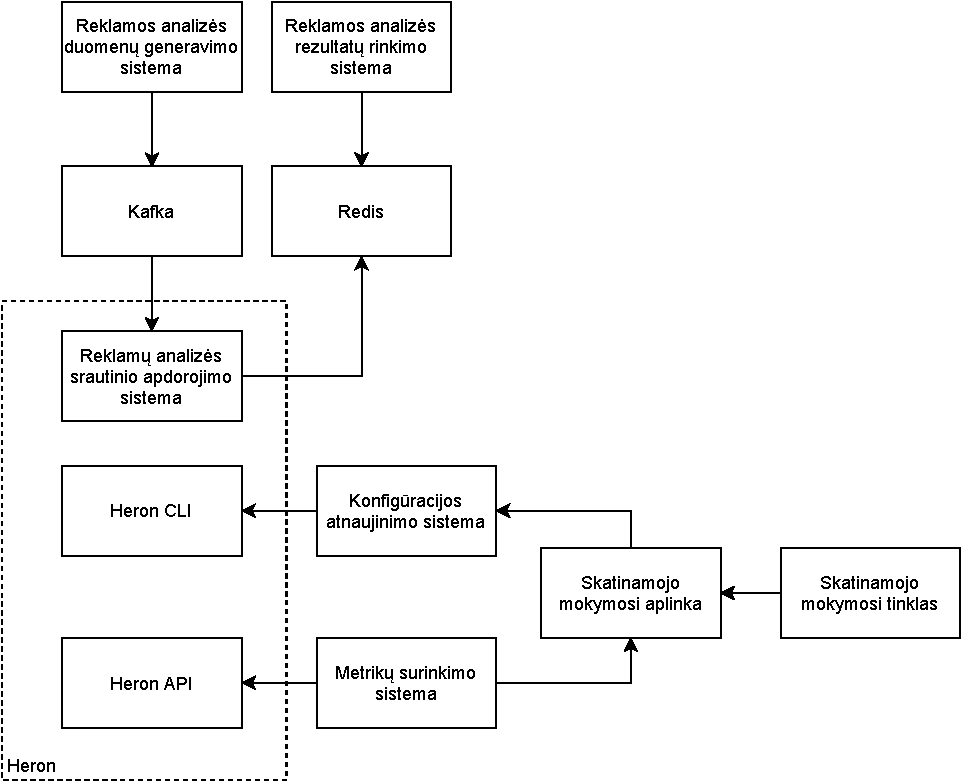
\includegraphics[width=14cm]{img/Experiment.pdf}
    \caption{Eksperimento sistemos architektūra}
    \label{experiment}
\end{figure} 

Sistemos, kurios reikalingos eksperimentui:
\begin{enumerate}
    \item Skatinamojo mašininio mokymosi sistema. Kadangi bus atlikti bandymai su dviem skatinamojo mokymosi algoritmais: Deep Q Network ir Soft Actor Critic, bus parašyti du mašininio mokymosi agentai naudojant Python su PyTorch biblioteka. Taip pat bus sukurta aplinka aprašanti srautinio apdorojimo sistemos būseną, veiksmų aibę ir konfigūracijos žingsnį. 
    \item Metrikų surinkimo sistema parašyta su Python naudojanti HTTP, kad gauti būsenos duomenis iš Heron API.
    \item Konfigūracijos atnaujinimo sistema parašyta su Python, kuri per Heron CLI pateikia atnaujintą konfigūraciją.
    \item Reklamų srautinio apdorojimo sistema parašyta su JAVA, gaunanti duomenis iš Kafka žinučių eilės ir sauganti rezultatus Redis duomenų bazėje.
    \item WordCount srautinio apdorojimo sistema parašyta su JAVA, pati generuojanti duomenis ir neperduodanti duomenis į išorę. 
    \item WordCount rezultatų surinkimo sistema parašyta su Python skaitanti vėlinimo metrikas iš Heron API ir sauganti rezultatus tekstiniame faile.
    \item Rezultatų apdorojimo sistema parašyta su Python, kuri surenka duomenis iš rezultatų failų, apdoroja juos ir grąžina skirtingų sprendimų diagramas.
    \item Reklamos analizės rezultatų rinkimo sistema parašyta su Clojure ir pateikta kartu su Reklamos analizės greitaveikos testu.
    \item Reklamos analizės duomenų generavimo sistema parašyta su Clojure ir pateikta kartu su Reklamos analizės greitaveikos testu.
\end{enumerate}

Kompiuterinės įrangos su kuria bus atliekamas eksperimentas parametrai:
\begin{itemize}
    \item Procesorius: Intel Core i7–5930k (6 branduoliai/12 gijų)
    \item Operatyvi atmintis: 64 GB (2666 MHz)
    \item Vaizdo plokštė: Nvidia GTX 1080Ti
    \item Operacinė sistema: Windows 10 Education
\end{itemize}

Kadangi Heron nepalaiko Windows sistemos visi tyrimai ir visos reikiamos posistemės leidžiamos naudojant Windows Subsystem Linux (toliau WSL) su Ubuntu 18.04. WSL yra suderinamumo sluoksnis naudojantis Linux branduolį per Hyper–V, kieno pagalba galima leisti programas skirtas Linux be emuliacijos neprarandant greitaveikos.

Pagrindinės programinės įrangos versijos:
\begin{itemize}
    \item Apache Heron: 0.20.3
    \item Kafka: 2.13
    \item Redis: 4.0.9
    \item Python: 3.6.9
    \item Java: 8
\end{itemize}
\subsection{Planuojamų eksperimentų apimtis}

Magistro darbe eksperimentai bus atliekami su keturiais skirtingais sprendimais:
\begin{itemize}
    \item Srautinio apdorojimo sistemos veikimas su standartine konfigūracija.
    \item Srautinio apdorojimo sistemos veikimas balansuojant ją naudojant sukurtą eksperimentinį sprendimą pagal apibrėžtą balansavimo algoritmą naudojant:
    \begin{itemize}
        \item REINFORCE algoritmą skatinamojo mokymosi posistemėje.
        \item Deep Q Network algoritmą skatinamojo mokymosi posistemėje.
        \item Soft Actor Critic algoritmą skatinamojo mokymosi posistemėje.
    \end{itemize}
\end{itemize}

Kiekvienas sprendimas bus testuojamas su dviem srautinio apdorojimo sistemų implementacijomis:
\begin{itemize}
    \item Reklamų analizės srautinio apdorojimo sistema.
    \item WordCount srautinio apdorojimo sistema.
\end{itemize}

Reklamų analizės sistema rezultatus talpina tekstini failą, kur kiekvienas įrašas yra vėlinimas milisekundėmis nuo paskutinio išsiųsto įrašo į žinučių eilę tam specifiniam kampanijos langui iki kol jis yra įrašomas į Redis duomenų bazę. WordCount sistemos rezultatai bus skaitomi tiesiai iš Heron platformos naudojant Heron API ir saugomi į failą tokiu pačiu formatu kaip ir reklamų analizės sistema, naudojant absoliutų vėlinimą gauta iš Heron API. 

Eksperimentai su visomis sistemomis bus vykdomi po 10 valandų, kadangi \cite{vaquero2018autotuning} straipsnio autoriai nustatė, kad jų balansavimo algoritmas konverguoja po maždaug 11 valandų. 
Gauti rezultatai iš failo bus skaitomi Python programa, kuri apdoroja duomenis į dvi grupes: visų sprendimų vėlinimą ir visų sprendimų vėlinimo 99–tą percentilę ir sugeneruoja linijines diagramas, kiekvienai vėlinimo grupei pagal sprendimą.

\sectionnonum{Rezultatai ir išvados}

\printbibliography[heading=bibintoc] 

\end{document}
